\documentclass[tikz,border=2pt]{standalone}
\usepackage{amsmath,amssymb}
\usepackage{tikz}
\usetikzlibrary{arrows.meta}

\begin{document}
% A normal vector n stands perpendicular to the plane: n . v = n . w = 0 for the direction
% vectors v and w, e.g. n = v x w in R^3.
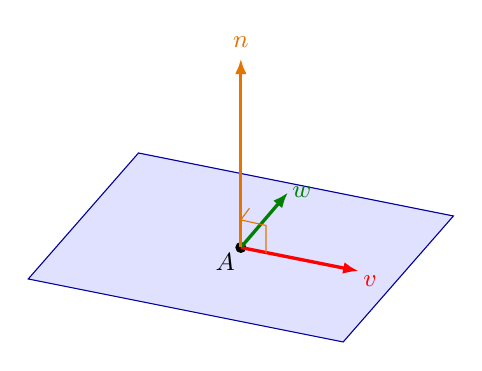
\begin{tikzpicture}[every node/.style={font=\small}, >={Latex[length=2mm]}]
	\fill[blue!12] (-1.6,0.2) -- (2.4,-0.6) -- (3.8,1.0) -- (-0.2,1.8) -- cycle;
	\draw[blue!60!black] (-1.6,0.2) -- (2.4,-0.6) -- (3.8,1.0) -- (-0.2,1.8) -- cycle;
	\coordinate (A) at (1.1,0.6);
	\fill (A) circle (2pt) node[below left, inner sep=2pt] {$A$};
	\draw[->, red, very thick] (A) -- (2.6,0.3) node[below right, inner sep=1pt] {$v$};
	\draw[->, green!50!black, very thick] (A) -- (1.7,1.3) node[right, inner sep=1pt] {$w$};
	\draw[->, orange!90!black, very thick] (A) -- (1.1,3.0) node[above] {$n$};
	\draw[orange!90!black] (1.1,0.95) -- (1.42,0.88) -- (1.42,0.53);
	\draw[orange!90!black] (1.1,0.95) -- (1.21,1.1);
\end{tikzpicture}
\end{document}
